\section{Decomposition theorem and applications}
\label{sec:dec-short}
In this section, we take a deeper look at decomposable permutations and investigate whether \greedy is ``decomposable'', in the sense that one can bound the cost of \greedy on input sequences by summing over local costs on blocks. Proving such a property for \greedy seems to be prohibitively difficult (we illustrate this in Appendix~\ref{sec:bad-example1}). Therefore, we propose a more ``robust'' but offline variant of \greedy which turns out to be decomposable. We briefly describe the new algorithm, and state the main theorems and three applications, leaving the details to Appendix~\ref{sec:decomposition}. 

\vspace{-0.06in}
\paragraph*{Recursive decomposition.}


We refer the reader to \S\,\ref{sec:results} for the definitions of blocks and recursive decomposition. Let $S$ be a $k$-decomposable permutation access sequence, and let $\tset$ be its (not necessarily unique) decomposition tree (of arity at most $k$).
Let $P$ be a block in the decomposition tree $\tset$ of $S$. Consider the subblocks $P_1, P_2, \dots, P_k$ of $P$, and let $\tilde{P}$ denote the unique permutation of size $[k]$ that is order-isomorphic to a sequence of arbitrary representative elements from the blocks $P_1, P_2, \dots, P_k$. We denote $P = \tilde{P}[P_1, P_2, \dots, P_k]$ a \emph{deflation} of $P$, and we call $\tilde{P}$ the \emph{skeleton} of $P$. Visually, $\tilde{P}$ is obtained from $P$ by contracting each block $P_i$ to a single point. We associate with each block $P$ (i.e.\ each node in $\tset$) both the corresponding rectangular region (in fact, a square), and the corresponding skeleton $\tilde{P}$ (Figure~\ref{fig_intro}). We denote the set of leaves and non-leaves of the tree $\tset$ by $L(\tset)$ and $N(\tset)$ respectively. %%%We remark that $L(\tset)$ contains only simple permutations.

Consider the $k$ subblocks $P_1,\ldots,P_k$ of a block $P$ in this decomposition, numbered by increasing $y$-coordinate. We partition the rectangular region of $P$ into $k^2$ rectangular regions, whose boundaries are aligned with those of $P_1,\ldots,P_k$. We index these regions as $R(i,j)$ with $i$ going left to right and $j$ going bottom to top. In particular, the region $R(i,j)$ is aligned (same $y$-coordinates) with $P_j$. 


\vspace{-0.06in}
\paragraph*{A robust version of \greedy.}
The main difficulty in analyzing the cost of \greedy on decomposable access sequences is the ``interference'' between different blocks of the decomposition. Our \agreedy algorithm is an extension of \greedy. Locally it touches at least those points that \greedy would touch; additionally it may touch other points, depending on the recursive decomposition of the access sequence (this a priori knowledge of the decomposition tree is what makes \agreedy an offline algorithm). The purpose of touching extra points is to ``seal off'' the blocks, limiting their effect to the outside.

We now define the concept of \emph{topwing}. The \textit{topwing} of a rectangular region $R$ at a certain time in the execution of \agreedy contains a subset of the points in $R$ (at most one in each column). A point is in the topwing if it forms an empty rectangle with the top left or the top right corner of $R$ (this definition includes the topmost touch point of the leftmost and rightmost columns of $R$, if such points exist in $R$). %, and 2) the topmost points in the left and right columns of $R$. 
When accessing an element at time $t$, \agreedy touches the projections to the timeline $t$ of the topwings of all regions $R(i,j)$ aligned with a block $P_j$ ending at time $t$ (this includes the region of $P_j$ itself). Observe that multiple nested blocks might end at the same time, in this case we process them in increasing order of their size. %%By touching these topwings, the interference between regions is limited, which allows us to decompose the cost of \agreedy. 
See Figure~\ref{fig_rgreedy} for an illustration of \agreedy.

\begin{figure}[h]
\centering
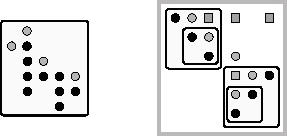
\includegraphics[scale=1.4]{fig_rgreedy.pdf}
\caption{Illustration of \agreedy. Left: region with points and \textit{topwing} highlighted. Right: a sample run of \agreedy on a $2$-decomposable input. Access points are dark circles, points touched by \greedy are gray circles, points touched by the \agreedy augmentation are gray squares. The access point in the topmost line completes the black square and also the enclosing gray square. The topwing of the black square consists of the black circle at position (1,6) and the gray circle at (3,5). Therefore the augmentation of the black square adds the gray square at (3,6). The topwing of $R(2,2)$ consists of the gray circle at (4,4) and hence the gray square at (4,6) is added. The topwing of the gray square consists of points (1,6) and (6,3); the point (4,4) does not belong to the topwing because (4,6) has already been added. Therefore, the gray square at (6,6) is added.}
\label{fig_rgreedy}
\end{figure}

\begin{theorem}[Decomposition theorem, Theorem~\ref{lem: main}]
\label{thm:main-sh} 

For any decomposition tree $\tset$ of a permutation $P$, the total cost of \agreedy is bounded as 
\vspace{-0.05in}
\[ \textsc{RGreedy}(P) \leq 4 \cdot \sum_{\tilde P \in N(\tset) }  \textsc{Greedy}(\tilde P) + \sum_{P \in L(\tset) } \textsc{Greedy}(P)+ 3n.\]
\end{theorem} 

  
\paragraph{Application 1: Cole et al.'s ``showcase'' sequences.} 
%In Cole et al.~\cite{finger1}, a showcase sequence is defined in order to introduce technical tools for proving the dynamic finger theorem. 
This sequence can be defined as a permutation $P = \tilde P[P_1,\ldots, P_{n/\log n}]$ where each $P_j$ is the permutation $(1,\ldots, \log n)$, i.e.\ a sequential access. 
It is known that \greedy is linear on sequential access, so $\textsc{Greedy}(P_j)  = O( \log n)$.  
%sequence for which \greedy has linear access cost, i.e.\ $|P_j| = \log n$, and $\textsc{Greedy}(P_j) = O(\log n)$. 
Now, by applying Theorem~\ref{thm:main-sh}, we can say that the cost of \agreedy on $P$ is $\textsc{RGreedy}(P) \leq 4 \cdot \textsc{Greedy}(\tilde P) + \sum_{j} \textsc{Greedy}(P_j) + O(n) \leq O(\frac{n}{\log n} \cdot \log (\frac{n}{\log n})) + \frac{n}{\log n}O(\log n) + O(n) = O(n)$. 
This implies the linear optima of this class of sequences.  

\paragraph{Application 2: Simple permutations as the ``core'' difficulty of BST inputs.}  

We prove that, if \greedy is $c$-competitive on simple permutations, then \agreedy is $O(c)$-approximate for all permutations. 

To prove this, we consider a block decomposition tree $\tset$ in which the permutation corresponding to every node is simple. Using Theorem~\ref{thm:main-sh} and the hypothesis that \greedy is $c$-competitive for simple permutations:

\[\textsc{RGreedy}(P) \leq 4c \cdot \sum_{\tilde P \in  N(\tset)} \opt(\tilde P) + c \cdot \sum_{P \in L(\tset)} \opt(P) +3n.\]

Now we decompose $\opt$ into subproblems the same way as done for \agreedy. We prove in \Cref{lem:decomp opt lower-bound} that $\opt(P) \geq \sum_{P \in \tset } \opt(P) - 2n$. Combined with Theorem~\ref{thm:main-sh} this yields $\textsc{RGreedy}(P) \leq 4c \cdot \opt(P) + (8c + 3)n$.  Using Theorem~\ref{thm:perm-all} we can extend this statement to arbitrary access sequences.



\paragraph{Application 3: Recursively decomposable permutations.} 
Let $X$ be a $k$-decomposable permutation. 
Then there is a decomposition tree $\tset$ of $X$ in which each node is a permutation of size at most $k$.
Each block $P \in L(\tset) \cup N(\tset)$ has $\textsc{Greedy}(P) = O(|P| \log |P|)  = O(|P| \log k)$.
By standard charging arguments, the sum $\sum_{P \in N(\tset) \cup L(\tset)} |P| = O(n)$, so the total cost of {\sc RGreedy} is $O(n \log k)$; see the full proof in Appendix~\ref{sec:decomposition}.  

We remark that the logarithmic dependence on $k$ is optimal (Proof in Appendix~\ref{sec:tight-block}), and that \greedy asymptotically matches this bound when $k$ is constant (Theorem~\ref{thm:main-noinitial}). 
